
\section{Hydropower Case and Implementation }
\label{case and implementation}

\subsection{Implementation environments}
\label{case:Implementation}
\subsubsection{Software}
\label{case:software}
All code is implemented and run in Python 3.8, except the parameter estimation of the price model, which is done in MATLAB2020b \cite{goodwin2013a}. In Python, the gurobipy package is used for the optimization models. A previous Python implementation of SDDP was also used \cite{ding2019python}.
\subsubsection{Hardware}
\label{case:hardware}
The computational tests are conducted on a system that allows for running up to 40 processes in parallel per node. In Table \ref{tab:hardware}, the relevant technical aspects of the hardware are given. 

\begin{table}[h]
\caption[Hardware specifications]{Hardware specifications}
\label{tab:hardware}
\centering
\begin{tabular} {l l}
\toprule
Specification &\hspace{5mm}Details\\
\midrule
Node System & \hspace{5mm} Dell PowerEdge R640\\
Node CPU: & \hspace{5mm} 2x 2.4GHz Intel Xeon Gold 5115 CPU – 10 core\\
Node RAM: & \hspace{5mm} 96Gb\\
\bottomrule
\end{tabular}
\end{table}
\label{computational_study:the case}


\subsection{Matre Haugsdal and Vemundsbotn}
\label{compuational_study:example_system}
This paper is written in cooperation with a major Norwegian hydropower producer. They have provided data for one of their hydropower systems. Matre Haugsdal and Vemundsbotn are power plants in western Norway. The plants are parts of the more extensive system of interconnected reservoirs built around the Matre watercourse. Together they produce enough electricity to cover the needs of more than 50k households. An overview of the system's layout as modelled can be seen in Figure \ref{fig:reservoir_overview}, and the publicly available technical specifications for the two production plants are given in Table \ref{tab:plant_specifications}.

\begin{figure}[H]
    \centering
    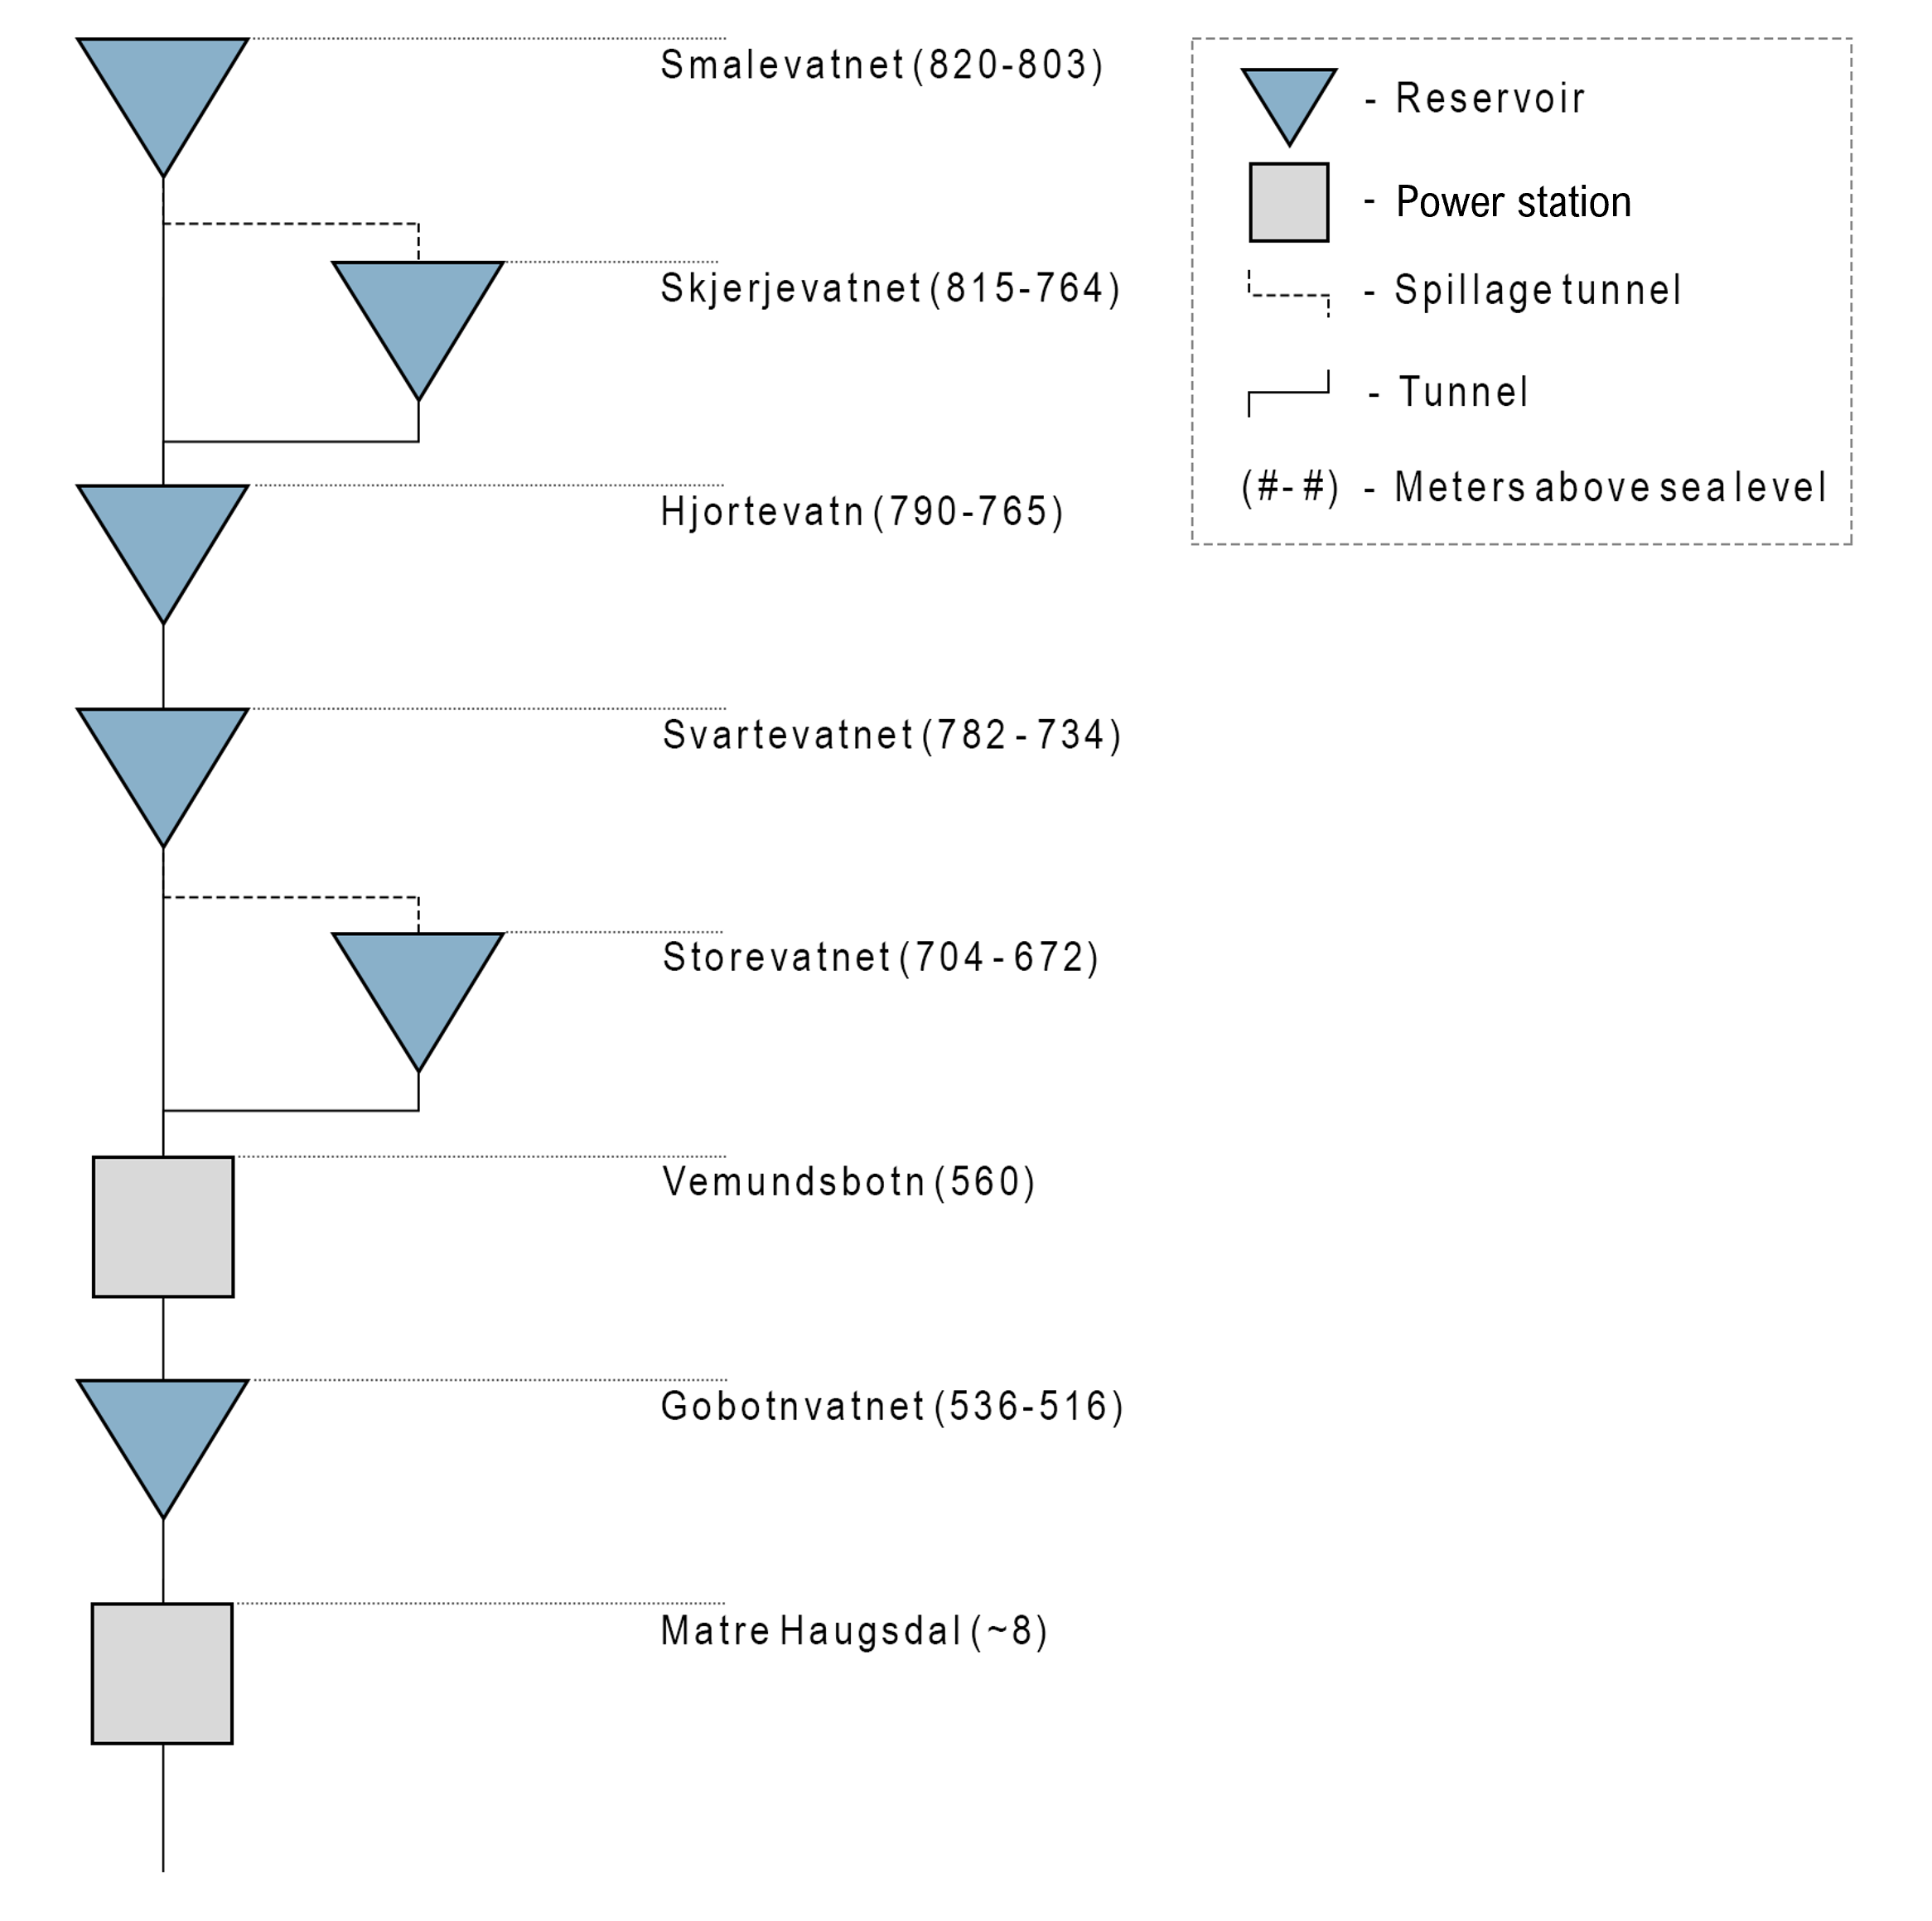
\includegraphics[width=1\textwidth]{reservoir figure.png}
    \caption[Reservoir overview]{Matre Haugsdal and Vemundsbotn, with connected reservoirs.}
    \label{fig:reservoir_overview}
\end{figure}

\begin{table}[H]
    \caption{Specifications for plants in the considered system}
    \label{tab:plant_specifications}
\centering
    \begin{tabular}{ l  c  r }
        \toprule
        &  Matre Haugsdal & Vemundsbotn\\ \midrule
        Build year &  2016 &  1976\\ 
        Turbines & 2 & 1 \\ 
        Production capacity [$MW$] & 180 & 45 \\ 
        Elevation  [$m$] & 537 & (164 / 242)$^*$  \\ 
        Head difference [$m$] & 20.5 & (32 / 48)$^*$ \\ 
        %Energy coefficient [$MJ/m^3$] & 1.2 & (0.395 / 0.55)$^*$\\
        \midrule
        \footnotesize$^*$Two connected reservoirs (Storevatnet/Svartevatnet)\\ \bottomrule

    \end{tabular}
\end{table}


Table \ref{tab:reservoir_specifications} shows the average annual inflows for each reservoir, along with their respective volumes and discharge capacities. A glance at the data shows that the reservoirs are of a ``fast" nature, meaning that the inflow to the reservoirs is relatively high compared to the storage capacity. We were not given any specified minimum discharge for the reservoirs in question, and thus, no lower bound is set for the model. Furthermore, the water level regulations for the reservoirs do not vary with season, but are constant throughout the year. 

\begin{table}[H]
    \caption{Reservoir specifications}
    \label{tab:reservoir_specifications}
\centering
    \begin{tabular}{ l  c  c  r}
        \toprule
        Reservoir &  Volume [$Mm^3$] & Inflow [$Mm^3/yr$] & \textcolor{red}{Max. Discharge} [$m^3/s$]\\[1mm] \midrule
        Gobotvatn &  22.0 &  134.6 & 37.6\\ 
        Storevatn & 23.3 & 57.6 & 18.0\\ 
        Svartevatn & 60.8 & 66.8 & 23.6\\ 
        Skjerjevatn  & 70.5 & 61.3 & 22.0 \\ 
        Hjortevatn & 10.7 & 60.9 & 10.0 \\ 
        Smalevatn & 13.1 & 96.5 & 19.8 \\ \bottomrule

    \end{tabular}
\end{table}  

\subsection{Price and Inflow Data}
\label{case:price}
Our price model uses futures data, and to generate the smoothed future curves, we use futures price data for the trading period 2006--2018, retrieved from Montel. The price simulations start 1 January 2019. The data is given per trading day, with closing prices for monthly, quarterly, and annual delivery for up to three years ahead. 
To fit the inflow model, we use time series inflow data for the reservoirs. The inflow data series provided are of hourly resolution in the period 2009--2019. 
